% !TeX spellcheck = da_DK
Dette afsnit fokuserer på designet af den robot der har til opgave at navigere rundt i et område for kortlægge det. 

Først vil det blive beskrevet hvordan selve robotten er bygget op med LEGO, og derefter hvordan motorer og sensorer er sat på robotten.

\begin{figure}
\centering
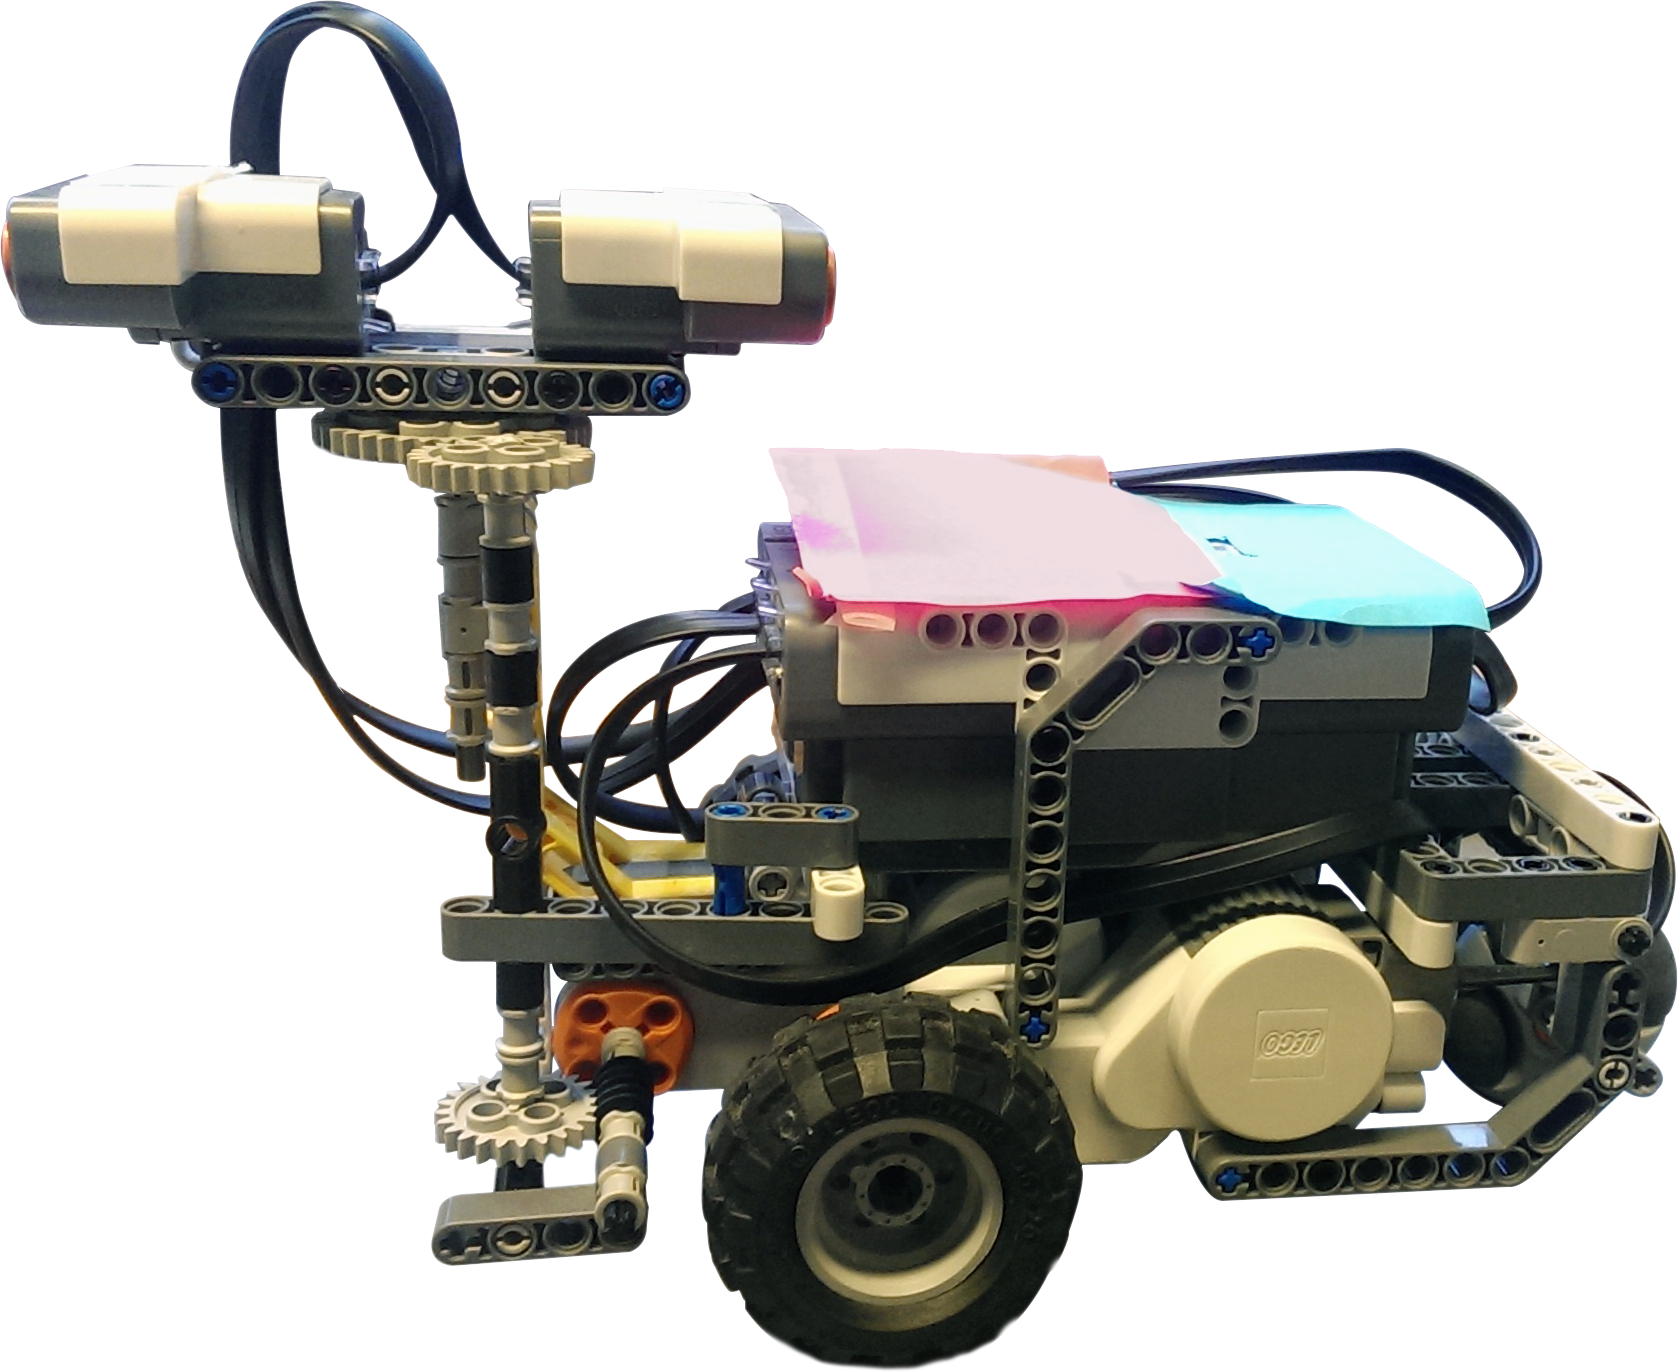
\includegraphics[width=0.6\textwidth]{whalle}
\caption{Endelige design af vores robot.}
\label{robot:opbygning}
\end{figure}




\subsection{Kroppen}
Kroppen er den centrale komponent, hvor motorene, som styrer henholdsvis hjulene og rotation af sensorerne, er bygget på. 
Samtidig fungere den som det, der "holder robotten sammen".
Desuden er NXTen også en central del af denne konstruktion.
Placeringen af denne er primært i forhold til funktionelle behov, da der på fronten er knapper til at tænde/slukke og vælge indstillinger med.
Dens placering gør det også nemt at få adgang til dens porte for tilslutning af motor, sensor, opladning samt tilslutning af PC for opdatering af software med mere.

\subsection{Fremdrift}
Robotten er konstrueret med et \textit{aktivt} hjulsæt, der både giver fremdrift og styring.
Denne funktionalitet opnås ved, at hvert hjul (på hver side af robotten) har sin egen motor, således der kan angives både positiv og negativ fremdrift uafhængigt af hvert hjul.
Dette design gør det muligt at rotere robotten omkring sin egen akse for maksimal mobilitet -- selv på et begrænset område.
Foruden det forreste hjulsæt, er der bagerst på robotten monteret et 'baghjul', hvis eneste funktion er at balancere/stabilisere robotten.
Valget af et hjul til at udføre en sådan funktion er forholdsvis begrænset i \lego, hvorfor valget faldt på et "slæbehjul" med en masse ruller, der gør det muligt for hjulet at rotere i alle retninger.

\subsection{Sensorer}
Den egentlige funktion af robotten er at tage afstandsmålinger til objekter indenfor sensorernes rækkevidde.
Placeringen af sensorerne er derfor ikke kritisk, da de højst vil give en forskydelse af konstant faktor relativ til robottens midte fra deres placering i fronten.
Vigtigere er, at der er 360\degree~udsyn når de roterer, og at robotten ikke er i vejen for målingerne, hvilket er løst ved at montere sensorerne højere end resten af robotten. 

I testen af afstandssensorer (se \cref{sensor:sammenligningIRvsSonar}) viste det sig at de to sensortyper, infrarød og ultrasonisk, havde sammelignelig præcision, og valget mellem disse to afhænger da af behovet for rækkevidde. 
Den infrarøde sensor kan måle præcist tæt på, mens den ultrasoniske kan måle præcist langt væk.
Til robotten blev det valgt at montere to ultrasoniske sensorer, da det ikke er lige så brugbart at vide tæt robotten er på en mur, som det er at se at der er en mur langt væk når der kortlægges.
